%\documentclass[aps,prl,reprint,twocolumn,superscriptaddress,sort&compress,10pt]{revtex4-1}  % for review and submission
% \documentclass[aps,preprint,12pt]{revtex4-1}  % for review and submission
%\documentclass[aps,twocolumn,floatfix,prl,10pt]{revtex4-1}
%\documentclass[letterpaper,10pt,prl,twocolumn,aps]{revtex4-1}
%\documentclass[aps,preprint,floatfix,prl]{revtex4-1}
\documentclass{jfm}
\usepackage{amsmath}
\usepackage{amsfonts}
\usepackage{amssymb}
\usepackage{graphicx}
\usepackage{booktabs}
\usepackage{color}
\usepackage{longtable}
\usepackage{array}
\usepackage{amssymb}
\usepackage[usenames,dvipsnames,svgnames,table]{xcolor}

\graphicspath{ {../Paper/images/}{../Paper/images/Growth_Rate_Cont_Plots/} }
\newcommand{\bx}{{\boldsymbol{\hat{x}}}}
\newcommand{\bn}{{\boldsymbol{\hat{n}}}}
\newcommand{\bt}{{\boldsymbol{\hat{t}}}}
\newcommand{\bu}{\mathbf{u}}
\newcommand{\grad}{\mathbf{\nabla}}
\newcommand{\del}{\partial}
\newcommand{\hg}{h_g}
%\newcommand{\Rey}{{R}}
\newcommand{\Ndg}{\tilde{N}_g}
\newcommand{\monami}{\textit{monami}}
\newcommand{\ubl}{U_\text{bl}}
\newcommand{\words}[1]{\textbf{(#1)~}}
% \newcommand{\words}[1]{{}}

\newcommand{\ReyNdg}{{\Rey\Ndg}}

\definecolor{tableShade}{gray}{0.8}
\title{\textit{Monami} as an oscillatory hydrodynamic instability in a submerged sea grass bed}
\author{Ravi Singh}
\affiliation{Brown University, Providence RI 02912 USA}
% \author{L. Mahadevan}
% \affiliation{Harvard University, Cambridge MA 02138 USA}
\author{M. M. Bandi}
\affiliation{OIST Graduate University, Okinawa 904-0495, Japan}
\author{Amala Mahadevan}
\affiliation{Woods Hole Oceanographic Institution, Woods Hole MA 02543 USA}
\author{Shreyas Mandre}
\affiliation{Brown University, Providence RI 02912 USA}


\begin{document}
\maketitle

\begin{abstract}
The onset of \monami ~-- the synchronous waving of sea grass beds driven by a steady flow -- is modeled as a linear instability of the flow. Our model treats the drag exerted by the grass in establishing the steady flow profile, and in damping out perturbations to it. This damping leads to a finite threshold flow for the instability, which agrees with experimental observations. This role of vegetation drag differentiates our mechanism from the previous hypothesis that the Kelvin-Helmholtz instability underlies \monami.
\end{abstract}

\maketitle
\section{Introduction}
Sea grasses exhibit a rich set of dynamical behavior due to their collective interaction with fluid flows.  
The hydrodynamic processes resulting from this behavior influence many environmental processes such as sedimentation, transportation of dissolved oxygen, plant growth, and biomass production  \cite{Fonseca87,Grizzle96,Nepf99,Nepf2012}. 
One such response of the submerged grass beds to steady currents is the formation of coherent large amplitude oscillations, known as \monami ~\cite{AckermanOkubo93}.  
In this letter, we provide a hydrodynamic mechanism for the onset of these coherent oscillations.

Current explanations of \monami ~invoke the existence of a free shear layer at the top of the grass bed (henceforth called grass top) due to vegetation drag  \cite{Ikeda96,Ghisal02,Raupach96}. 
Its instability, through a mechanism similar to the Kelvin-Helmholtz instability, is thought to lead to coherent eddies over the grass bed, and drive large amplitude synchronous oscillations.
This model has been applied to predict the observed frequency of \monami~and to understand transport in the seagrass bed \cite{Nepf00,Ghisal02,Nepf04,Okamoto12}.

However, several aspects of this explanation remain unsatisfactory: 
(i)   The velocity profile of the free shear layer is assumed \textit{ad hoc} to be piecewise linear \cite{Delangre06} or hyperbolic tangent \cite{Ghisal02,Raupach96}. 
(ii)  The role of drag in damping the coherent perturbations to the shear profile is sometimes ignored \cite{Raupach96}. 
(iii) No existing theory explains the threshold flow speed, observed in the lab \cite{Ghisal02} and the field \cite{Grizzle96}, below which \monami ~is not observed.
(iv)  The thickness of the free shear layer is in many cases comparable to the unvegetated water depth, and therefore inconsistent with the definition of the free shear layer.
Here we present a mathematical model for the linear instability that accounts correctly for these effects, while also explaining lab experiments and field observations.

\section{Mathematical model}
Although \monami ~is manifest in the motion of the grass, the drag exerted by the grass bed on the flow is central to the hypothesized instability. 
The instability and the resulting flow structures persist in lab experiments even when flexible grass mimics are replaced by rigid dowels \cite{Ghisal02,Nepf06}. 
Therefore, to develop the essential mathematical model, we assume the grass blades to be rigid, on average oriented vertically.
We show that the drag of the grass results in an instability mode different from the Kelvin-Helmholtz instability.
\begin{figure}
\centerline{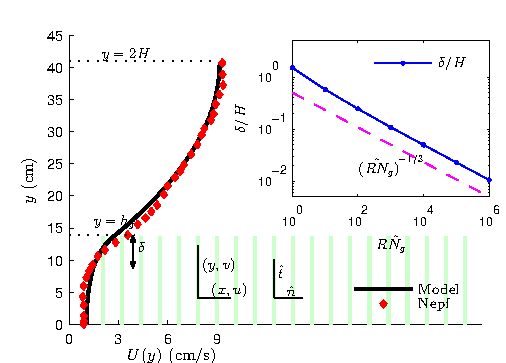
\includegraphics[scale=1]{Grass_Base_Nepf_shear}}
% 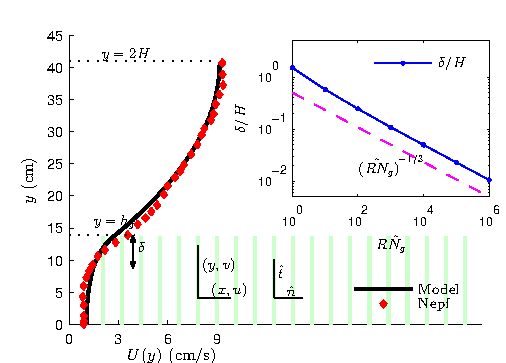
\includegraphics[width=15cm]{Grass_Base_Nepf_shear}
\caption{
Schematic setup and comparison of our steady flow profile with that from the experiments in ref. \cite{Nepf04} (Case I from Table 1) %  with 1250 plants/m$^2$, plant height = 13.7$\pm 0.2$ cm and blade width of 0.64 cm)
 and its approximation with $U_0=7.28$ cm/s and $\delta = 5.02$ cm in our model. The grass extends up to $y=\hg$ in the water column of depth $2H$. 
The steady velocity profile can be decomposed into a parabolic profile in the unvegetated region, a uniform profile deep within the vegetation, and a boundary layer of thickness $\delta$ near the grass top. 
The dependence of the boundary layer thickness (estimated as $|U/U_y|$ at $y=\hg$ from the numerical solution of \eqref{base_equ}) on the vegetation density parameter $\ReyNdg$ is shown in the inset.
}
\label{basicflow}
\end{figure}
\begin{figure}
\begin{center}
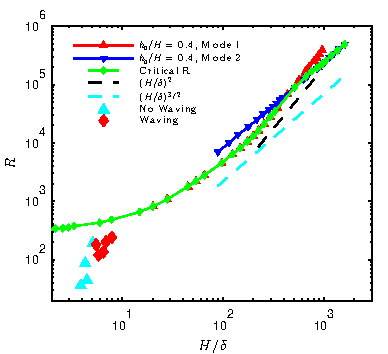
\includegraphics[scale = 0.95]{new_graph_R_vs_delta}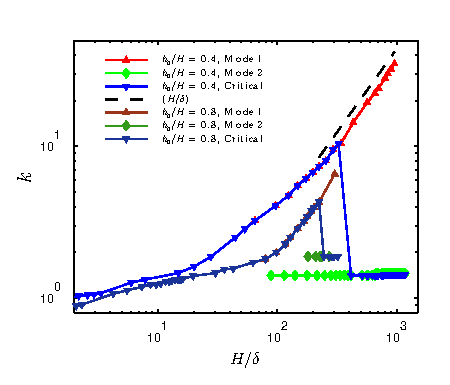
\includegraphics[scale = 0.95]{new_graph_K_vs_delta}
% 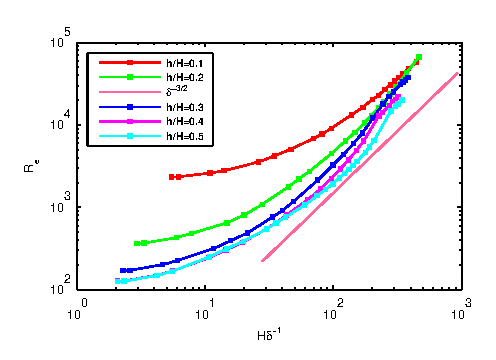
\includegraphics[width=12cm]{Critical_Re_vs_delta_noshear} \\
% \vspace{-6mm} \hspace{-5mm}
% 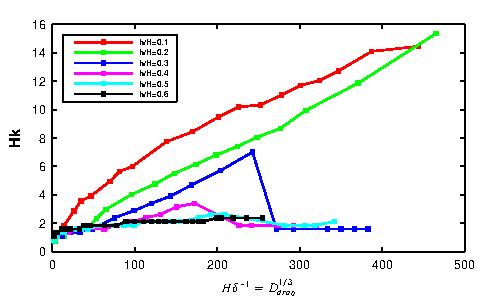
\includegraphics[width=12cm]{K_vs_shear_width_noshear}
\end{center}
\caption{
Critical Reynolds number (top) and the corresponding marginally stable wave number (bottom) for different submergence ratio as a function of vegetation density parametrized by the boundary layer thickness. 
Parameters from experiments reported in ref. \cite{Ghisal02} to exhibit or suppress synchronous waving are also included in the top panel. 
Inset compares experimental observations of the experimentally measured dominant frequency $f_o$ (in Hz) with the predictions $f_p=\text{Im}(\sigma)$ from the solution of ~\eqref{Orr-somerfield}. 
The experimental data in the inset is obtained from refs. \cite{Ghisal02} (Ghisalberti) and \cite{Vivoni98} (Vivoni). 
In order to estimate the $\Rey$ for these experiments, a representative value of $\mu=0.1$ Pa~s was assumed.
}
\label{Re_vs_delta}
\end{figure}

The drag exerted by the vegetation, assumed dense, is modeled by a continuous body force $\mathbf{f}$.
This drag enters the fluid mass and momentum balance equations as 
\begin{equation}
\grad\cdot\bu = 0,\hspace{3mm} \rho \left(\bu_{t}+\bu.\grad\bu \right) = -\grad p+\mu\grad^{2}\bu +\mathbf{f}+\rho\mathbf{g}
\label{navier-stokes}
\end{equation}
where $\rho$, $\bu$, and $p$ are the fluid density, velocity, and pressure respectively, $\mu$ the dynamic eddy viscosity and $\mathbf{g}$ the acceleration due to gravity. 
The Reynolds number of the flow based on the scale of the grass blade is $O(10^2-10^3)$; therefore, neglecting the skin friction, we model it as the form drag on the vegetation, $\mathbf{f}=N_g C_N \rho u |u| d\bx$ \cite{Nepf99,Nepf00,Nepf04}, where  $N_g$ is the blade number density per unit horizontal area, $C_{N}$ the drag coefficient, and $d$ the average blade width projected perpendicular to the flow. 
In the interest of simplicity, we model the turbulence using an eddy viscosity; see \S\ref{subsec:turbulencemodel} for a detailed discussion. 
In the field, both $C_N$, $N_g$ and $\mu$ vary with position, but we do not expect these variations to be central to the instability mechanism, and therefore take them to be constants. 
Based on previous experiments \cite{Vivoni98,Nepf00}, we take $C_N = 1$.

\begin{figure*}
 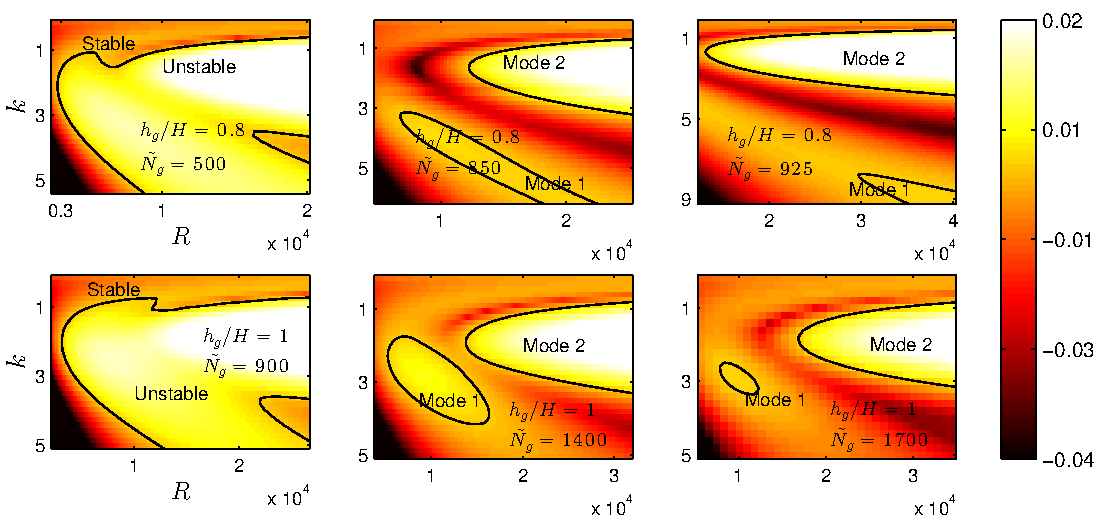
\includegraphics[width=\textwidth]{SetAll_imgsc}
%\end{figure}
%\begin{figure*}
%\begin{tabular}{cccc}
%{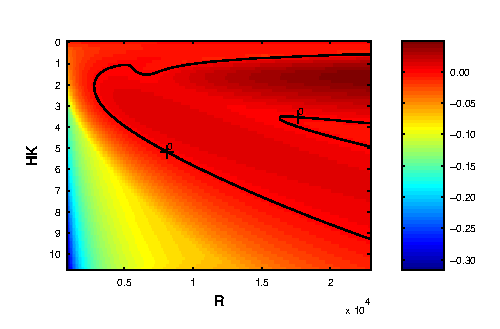
\includegraphics[height = 4cm, width = 5.8cm]{Set4_dens28_imgsc}} &
%{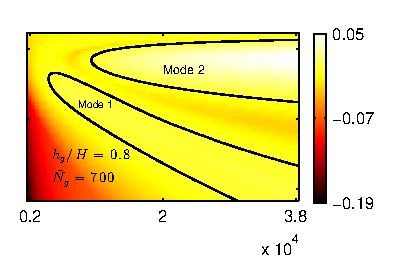
\includegraphics[scale = 0.67]{Set4_dens30_imgsc}} &
%{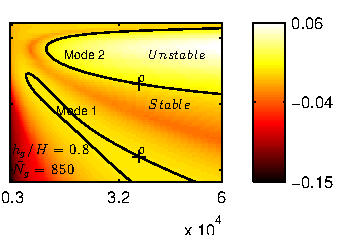
\includegraphics[height = 4cm,width = 5.8cm]{Set4_dens32_imgsc}} &
%{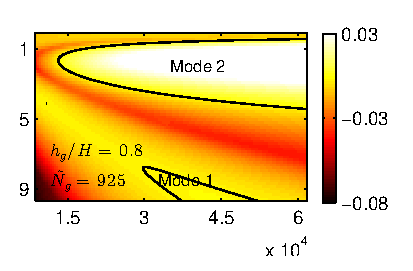
\includegraphics[height = 4.15cm,width=6.5cm]{Set4_dens34_imgsc}} \\
%{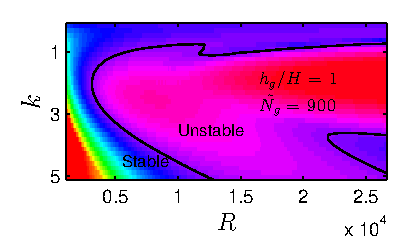
\includegraphics[height = 4cm, width = 5.8cm]{Set5_dens38_imgsc}} &
%{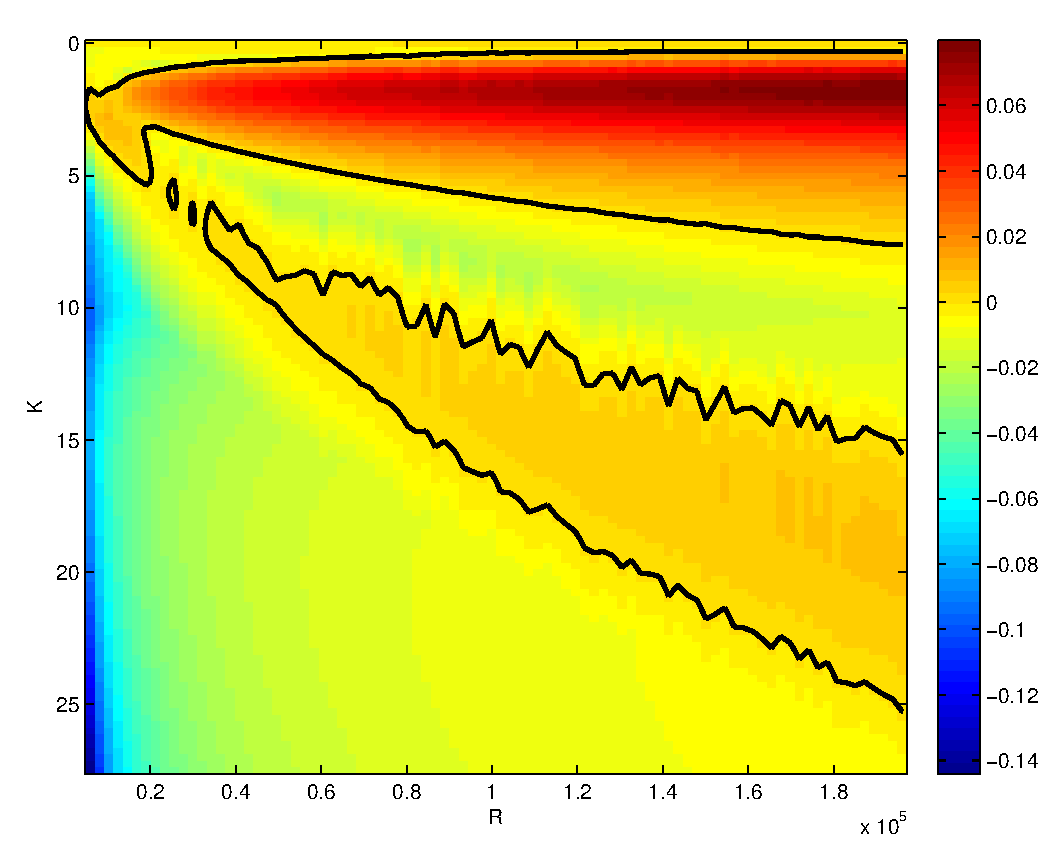
\includegraphics[scale = 0.67]{Set5_dens40_imgsc}} &
%{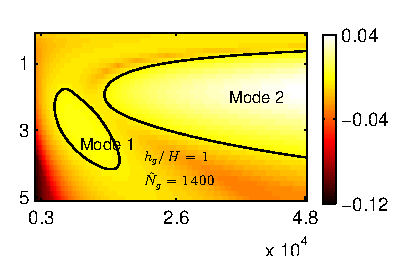
\includegraphics[height = 4cm, width = 5.8cm]{Set5_dens42_imgsc}} &
%{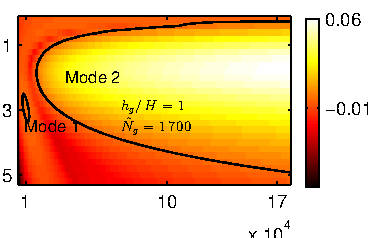
\includegraphics[height = 4.15cm,width=6.5cm]{Set5_dens46_imgsc}} \\

%{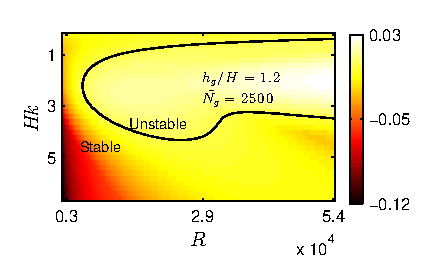
\includegraphics[scale = 0.67]{Set6_dens32_imgsc}} &
%{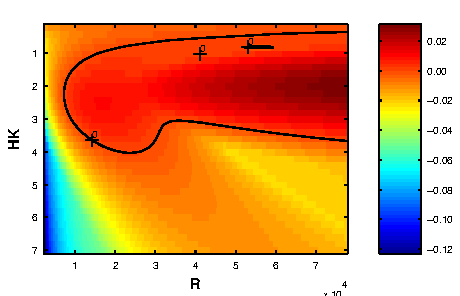
\includegraphics[scale = 0.67]{Set6_dens34_imgsc}} &
%{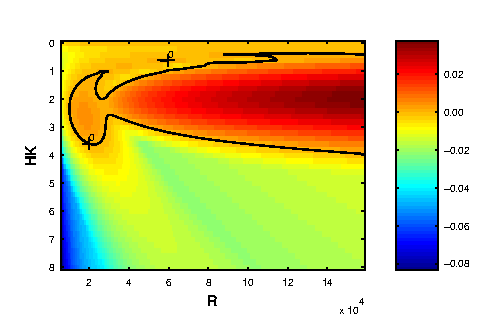
\includegraphics[scale = 0.67]{Set6_dens36_imgsc}} &
%{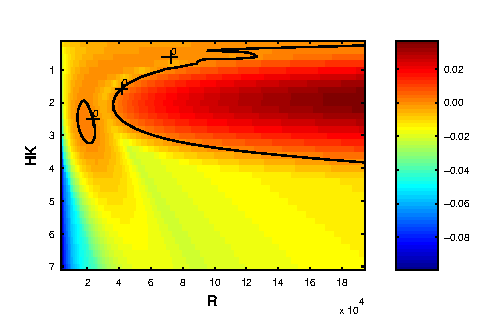
\includegraphics[scale = 0.67]{Set6_dens38_imgsc}}
%\end{tabular}
\caption{
$Re(\sigma)$ and the neutral curve ($Re(\sigma)$=0) as function of wavenumber and $\Rey$ for parameters shown in the corresponding panel.  
As $\Ndg$ increases, the unstable region splits into two labeled as ``Mode 1'' and ``Mode 2''. 
For $\Ndg$ below (above) a critical value, Mode 1 (Mode 2) sets the threshold $\Rey$.
}
\label{K_Re_sigma_set3}
\end{figure*}

\section{Linear stability analysis}
We first calculate the fully developed steady solution $\bu = U(y)\boldsymbol{\hat{x}}$ of ~\eqref{navier-stokes} driven by constant pressure gradient $dP/dx$, satisfying
\begin{equation}
 -\frac{dP}{dx}+\mu U''(y) +S(y) \rho C_N d N_gU |U|=0
\label{base_equ}
\end{equation}
where $S(y)=1$ for $0<y<\hg$ and $S(y)=0$ for $\hg< y< 2H$. 
Eq. \eqref{base_equ} is solved subject to no shear at the boundaries, i.e., $U'(0) = U'(2H) = 0$.
The former arises for dense vegetation because the shear stress exerted by the bottom surface is expected to be negligible compared to the vegetation drag~\cite{Nepf00}, whereas the latter models the free interface. 
A comparison of the steady flow profile from the solution of ~\eqref{base_equ} with experimental measurements is shown in Fig.~\ref{basicflow}.
The profile $U(y)$ has three distinct regions.
Within vegetation, it is approximately uniform with $ U(y) \approx U_g = \sqrt{\frac{dP/dx}{\rho C_N dN_g}}$, arising from balancing the drag with pressure gradient. 
Outside the vegetation, the velocity has a simple parabolic profile. % due to the balance between viscous forces and the pressure gradient. 
At the grass top, continuity of shear stresses results in a boundary layer of thickness $\delta$. 
Denoting $\ubl$ to be the velocity scale in the boundary layer, and $U_0 = {(dP/dx)~H^2}/{\mu}$ the velocity scale in the unvegetated region, the balance between viscous forces and vegetation drag implies $(\mu \ubl/\delta^2 \sim \rho C_N d N_g \ubl^2)$, and the continuity of shear stress across the grass top implies $(\ubl/\delta \sim U_0/H)$.
Solving for $\delta$ and $\ubl$ yields $\delta/H = \ubl/U_0=(\ReyNdg)^{-1/3}$, where $\Ndg = \left(C_N d H N_g\right)$ is the vegetation frontal area per bed area, and $\Rey=\rho U_0 H/\mu$ is the Reynolds number of the flow. 
A numerical estimate of $\delta$ ($U/U_y$ at $y=\hg$) is compared with this prediction in Fig. \ref{basicflow} (inset).
Because this boundary layer develops independent of the influence of the boundaries, we identify it to be analogous to the free shear layer \cite{Ghisal02,Nepf04} in the previous explanation of \monami.
This dependence of $\delta$ on $N_g$, verified in Fig.~\ref{basicflow}, gives us a way to systematically investigate the effect of the shear layer thickness on the instability mechanism.
The figure also shows that the asymptotic regime of a thin boundary layer is expected to hold for $\ReyNdg \gtrsim 100$. In this notation, $U_g/U_0 = (\Rey \Ndg)^{-1/2}$ (used for deriving \eqref{eqn:mode2asymp}). 

Next we substitute $\bu = (U+\tilde{u}, \tilde{v})$, $p=P+\tilde{p}$ in ~\eqref{navier-stokes} and expand to linear order to investigate the evolution of small perturbations $(\tilde{u}, \tilde{v})$, which obey
\begin{equation}
\begin{split}
\rho(u_t+U u_x+vU_y) &= -p_x+ {\mu}\nabla^2u-2S\rho C_{N}dN_{g}Uu, \\
\rho(v_t+ Uv_x) &= -p_y+ {\mu}\nabla^2v, \hspace{0.3cm} \nabla\cdot\bu=0,
\end{split} \nonumber
\end{equation}
where the tilde are dropped.
These equations are non-dimensionalized using half channel height $H$, velocity $U_0$, and time $H/U_0$, leading to three non-dimensional parameters, \textit{viz.} $\Rey$, $\Ndg$, and the vegetation submergence ratio $\hg/H$. 
We also use $\delta/H$ in lieu of $\Ndg$ to parametrize the vegetation density and help elucidate the instability mechanism. 
Using a stream function $\psi$ with $u = \psi_{y}, v= -\psi_x$ to satisfy mass balance, we seek a solution of 
the form $\left(u,v,\psi \right)= \left(\hat u(y), \hat v(y), \phi(y) \right)e^{ikx+\sigma t}$ to obtain a modified Orr-Sommerfield equation \cite{Drazin81} 
\begin{equation}
\begin{split}
\left(D^2 -k^{2} \right)^2\phi &= \Rey \left[ \left({\sigma}+ikU\right) \left(D^2-k^2\right) -ikU_{yy}\right]\phi \\
&+\Rey \Ndg D\left(2 S U D \phi\right),
\label{Orr-somerfield}
\end{split}
\end{equation}
where $D=d/dy$, and subject to the boundary conditions $D\phi = D^2\phi = 0$ at $y=0$ and $y=2$. 
The growth rate $\sigma$ for a given wave number $k$ appears as an eigenvalue that allows a non-trivial solution $\phi$ of  \eqref{Orr-somerfield}.
We solve \eqref{Orr-somerfield} numerically for $\sigma$ and $\phi$.

\section{Results - unstable modes and critical parameters}
A threshold in $\Rey$, above which the flow is unstable (Re$(\sigma)>0$) for at least one $k$, emerges from the solution of ~\eqref{Orr-somerfield}. 
The dependence of this threshold $\Rey$, and the corresponding marginally stable wavenumber $k$, on $\delta/H$ and $\hg/H$ is shown in Fig.~\ref{Re_vs_delta}, and is found to compare well with experimental observations \cite{Ghisal02}.
The threshold $\Rey$ increases with the vegetation density, indicating a competition between the destabilizing shear in the flow, and the stabilizing effect of damping due to vegetation drag.
A similar conclusion was presented for an analogous problem (flow around an emergent (i.e., $\hg>2H$) sea grass patch), but by assuming $U(y)$ to be a tanh-profile, and neglecting the viscous term \cite{White07}.
Previous calculations for terrestrial grass either exclude the vegetation drag in their models \cite{Raupach96}, or assume the mean velocity profile \textit{ad hoc} \cite{Raupach96,Delangre06}.
A threshold flow condition is not reported previously either for terrestrial or submerged marine meadows.

The frequency (Im$(\sigma)$) of the fastest growing mode agrees well with observed frequencies -- frequency of \monami, maxima in the velocity spectra, and frequency of vortex passage in lab scale experiments \cite{Ghisal02} -- for cases where the vegetation was sufficiently dense to be modeled by a continuum drag field, as shown in the inset in Fig.~\ref{Re_vs_delta}. 
The experimentally observed \monami ~wavelengths are not available for comparison.

\begin{table*}
% \footnotesize
\rowcolors{3}{tableShade}{white}  %% start alternating shades from 3rd row
\renewcommand{\arraystretch}{1.2}
 \begin{tabular}{l|c|c|c}
			& Kelvin-Helmholtz 				& Mode 1 		& Mode 2 \\ \hline
 Base velocity profile 	& $U(y) = U_0 \tanh(y/\delta)$			& \multicolumn{2}{c}{Equation \eqref{base_equ}} \\
 Domain 		& $-\infty < y < \infty$			& \multicolumn{2}{c}{$-1<y<1$} \\
 Inflection point	& exists at $y=0$				& \multicolumn{2}{c}{$U''(y)$ discontinuous at $y=\hg$} \\
 Shear layer thickness	& $\delta$					& \multicolumn{2}{c}{$\delta \sim  H\left(\Rey \Ndg \right)^{-1/3}$} \\
 Linearized dynamics	& Equation \eqref{eqn:Rayleigh}		& \multicolumn{2}{c}{Equation \eqref{Orr-somerfield}} \\
 Dense grass limit &  no grass included & Equation \eqref{eqn:mode1asymp} & Equation \eqref{eqn:mode2asymp}  \\
 Critical parameters	& none						& $\Rey \propto \Ndg^{2}$ 	& $\Rey \propto \Ndg$ \\
 Most unstable $k$ as $\delta \to 0$	& $\propto H/\delta$		& $\propto H/\delta$	& $O(1)$ \\
 Mode localized?	& yes, near $y=0$				& yes, near $y=\hg$			& no, spans water column
 \end{tabular}
 \caption{Comparison between Kelvin-Helmholtz instability and the two unstable modes resulting from solution of \ref{Orr-somerfield}.}
 \label{tab:comparison}
\end{table*}
To better understand the instability mechanism, we consider the dependence of the fastest growing wavenumber on $\delta$.
The fastest growing wavenumber first increases proportional to $H/\delta$, but at a critical $\delta$ discontinuously jumps and remains $O(1)$ (see Fig.~\ref{Re_vs_delta}). 
To aid in explaining this behavior, we show heat maps of Re$(\sigma)$ as a function of $\Rey$ and $k$, for different $\hg/H$ and $\Ndg$ in Fig.~\ref{K_Re_sigma_set3}. 
The smallest $\Rey$ on the neutral curve (Re$(\sigma)=0$) sets the threshold. 
We observe that as $\Ndg$ increases, the unstable region splits into two; we refer to the region with the higher $k$ as ``Mode 1'', and the one with the lower $k$ as ``Mode 2''. 
The unstable region for Mode 1, depending on $\hg/H$ either recedes to higher $\Rey$ or shrinks to zero size, as the vegetation density increases, causing the most unstable mode to transition discontinuously.

\section{Discussion -- comparison of unstable modes with Kelvin Helmholtz}
The distinct asymptotic behavior of the two modes as $\Ndg \gg 1$ distinguishes it from the Kelvin-Helmholtz instability. 
\subsection{Mode 1}
Our numerical calculation show that Mode 1 asymptotically localizes to the boundary layer near the grass top, and exhibits highest growth for a for a perturbation of  $k \sim H/\delta$. We also observe that critcal Reynolds number above which perturbation become unstable scales as  $\Rey (\sim H/\delta)^2$ (or $\Rey \propto {\Ndg}^{2}$). The behavior of this critical Reynolds number can be understood by asymptotically estimating the size of various terms in boundary layer in ~\eqref{Orr-somerfield}. Using $D\sim H/\delta$, $\sigma \sim O(1)$, and $\ubl \sim \delta/H$; the magnitude of the advection term is $\Rey (H/\delta)^2$  (or $\Rey^{5/3} \Ndg^{2/3}$), and the viscous as well as vegetation drag term are $(\delta/H)^{-4}$ (or $(\Rey \Ndg)^{4/3})$. The advection term, viscous term and vegetation drag terms balances when $\Rey \sim (H/\delta)^2$ (or $\Rey \sim {\Ndg}^{2}$), confirming our numerical finding.
\newline
Inorder to further understand the mechanism of Mode-1, we rescale \eqref{Orr-somerfield} in the the boundary layer using $\eta = y/\delta$, 
$U(y) = (\delta/H)\bar{U}(\eta)$ and $k = (H/\delta) \bar{k}$, with these scalings ~\eqref{Orr-somerfield} simplifies to
\begin{equation}
\begin{split}
\left(\bar{D}^2 -\bar{k}^{2} \right)^2\phi &= (\Rey/\Ndg^2)^{1/3} \left[ \left({\sigma}+i\bar{k}\bar{U}\right) \left(\bar{D}^2-\bar{k}^2\right) -i\bar{k}\bar{U}_{\eta\eta}\right]\phi \\
&+\bar{D}\left(2S \bar{U} D \phi\right),
\label{eqn:mode1asymp}
\end{split}
\end{equation}

in a region of thickness O($\delta$) near $y=\hg$. Since $(\Rey/\Ndg^2)$ is the only remaining parameter in \eqref{eqn:mode1asymp}, the mode shape and soulution will converge in the limit of $R \sim \Ndg^2$, confirming our numerial finding which is shown in Fig \ref{Asymptotic_mode}. 
\newline
Since by increasing $\Rey$ in the above equation for a  fixed $\Ndg$ we recover the linearized dynamics of Kelvin-Helmholtz equation, signifying that Mode-1 is similar to Kelvin-Helmholtz instability. We can further corroborate this claim by observing that both Kelvin-Helmholtz and Mode-1 shows that (i) Critical wavenumber $k \sim O(H/\delta$, (ii) Strong shear in the boundary layer plays crucial role in the flow instability
(iii) Dominant mode of instability is localized near the boundary layer. 

%We expect identical asymptotic behavior for a fixed relative magnitude of the terms on the r.h.s. to those on the l.h.s. of \eqref{eqn:mode1asymp}, which is $(\Rey \delta/H)^{3/2}$ (or $\Rey/\Ndg^{1/2}$).
%Therefore the threshold obtained for Mode 1 is $\Rey \propto H/\delta$ (or $\Rey \propto \Ndg^{1/2}$) explaining the numerically observed asymptote (see Fig.~\ref{Re_vs_delta}). 
%This analysis also concludes that the mode structure is self-similar over the length scale $\delta$ for fixed $\Rey/\Ndg^{2}$; the verification of this idea is shown in Fig.~\ref{Asymptotic_mode} (inset).

\subsection{Mode 2}
The threshold condition for Mode 2 is numerically observed to be $\Rey \propto ({\delta}/{H})^{-3/2}$ (or $\Rey \propto \Ndg$) for $k\sim O(1)$, shown in Fig.~\ref{Re_vs_delta}, which can be understood by assuming $\Rey \gg 1$ but fixed $\Rey/\Ndg \sim O(1)$.
% Note that for large $\Ndg$, the non-dimensional steady flow velocity inside the vegetation is $U_g \sim (\Rey \Ndg)^{-1/2}$. 
In this limit, the non-dimensional flow in the grass bed is $U\sim (\Rey \Ndg)^{-1/2} \ll 1$, and therefore $\sigma + ikU \approx \sigma$ to leading order. 
Furthermore, $U_{yy}$ decays to zero outside the boundary layer. 
Outside the grass, the turbulent viscous stress term is negligible compared to the inertial term. Thus, \eqref{Orr-somerfield} simplifies to 
\begin{subequations}
\begin{align}
% \begin{split}
\sigma\left(D^2-k^2\right)\phi = -2{(\Ndg/\Rey)^{1/2}}D^2\phi,  \quad &\text{ for } y<\hg  \label{eqn:mode2asympa} \\
\left(\sigma+ikU\right) \left(D^2-k^2\right)\phi =  ikU_{yy}\phi, \quad &\text{ for } y>\hg. \label{eqn:mode2asympb}
% \end{split}
\end{align}
\label{eqn:mode2asymp}
\end{subequations}

\begin{figure}
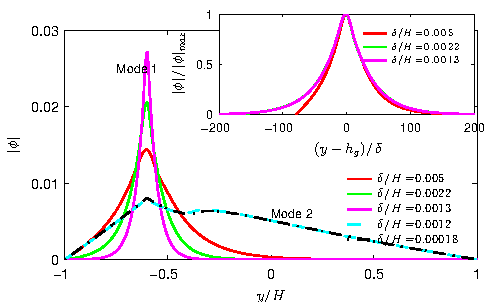
\includegraphics[]{Asymptotic_noshear}
% 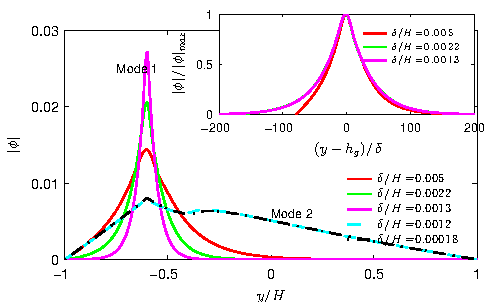
\includegraphics[width=12cm]{Asymptotic_noshear}
\caption{
Plot of the neutral Mode 1 (solid) and Mode 2 (dashed) shape $|\phi|$ in the limit of small $\delta/H$ for $\hg/H=0.2$. 
% Mode 1 is shown in solid and Mode 2 is shown in dashed. The parameters for Mode 2 shapes are chosen such that $\Rey \gg 1$, $\Ndg \gg 1$ (specified in terms of $\delta/H$) but $\Rey/\Ndg = O(1)$. 
The approach of mode shapes to each other for these small values of $\delta/H$ indicates that the dense vegetation asymptote is reached. 
Mode 1 shapes appear self-similar in shape as $\delta\to 0$.
Inset shows rescaled $|\phi|$ for Mode 1 as a function of $(y-\hg)/\delta$ approach a universal shape, indicating that an asymptotic limit has been reached. 
% The limit is not yet reached for the case $\delta/H = 0.005$ due to the influence of bottom boundary; the vegetation height in this case is comparable to the boundary layer thickness.
}
\label{Asymptotic_mode}
\end{figure}
The only remaining parameter in \eqref{eqn:mode2asymp} is $\Rey/\Ndg$. 
For fixed $\Rey/\Ndg$, the mode shape converges in the aforementioned limit, in agreement with our numerical results shown in Fig.~\ref{Asymptotic_mode}.
This convergence indicates that we have identified the correct asymptotic limit to investigate Mode 2.

The parameter $\Rey/\Ndg$ therefore sets the threshold, justifying the numerically observed asymptotic behavior $\Rey \propto \Ndg$ (or $\Rey \sim ({\delta}/{H})^{-3/2}$; see Fig.~\ref{Re_vs_delta} for comparison with numerical results).
The structure of this mode in the aforementioned limit is such that $\phi$ is continuous at $y=h_g$, but $D\phi$ undergoes a rapid transition there on the scale of boundary layer thickness $\delta$.
The eigenvalues and the mode shape are otherwise independent of $\delta$, and therefore we conclude that the boundary layer only plays a secondary role of regularizing the discontinuity in tangential velocity arising at $y=\hg$ in this instability mechanism.
% We interpret Mode 2 as the instability of an inviscid fluid, with the vegetation modeled by a continuum drag field, and for which the boundary layer near the grass top plays no role. 
% On the other hand, Mode 1 asymptotically localizes to the boundary layer near the grass tip, and exhibits a different asymptotic behavior with $k \sim O(H/\delta)$, and $\Rey \sim (H/\delta)$ (or $\Rey \propto {\Ndg}^{1/2}$) at the threshold. 

\subsection{Comparison with Kelvin-Helmholtz}
Table \ref{tab:comparison} compares the two modes to each other, and to the Kelvin-Helmholtz instability. 
Because the eigenfunction of Mode 1 is localized over a length scale $\delta$, it may be interpreted as the instability of the flow in the boundary layer, whereas Mode 2 may be understood as the instability on the scale of the water column. 
Mode 1 appears to be superficially similar to the Kelvin Helmholtz mechanism, whereas Mode 2 arises purely from the interaction between the unvegetated water column and the flow through the vegetation. 
The appearance of the vegetation drag parameter in the dominant balances represented by ~\eqref{eqn:mode1asymp} and ~\eqref{eqn:mode2asymp}, and the resulting threshold criteria demonstrates its role in setting the threshold, and in distinguishing them from the Kelvin-Helmholtz instability.
% Vegetation drag plays a dominant role in the mechanism for both the modes, which distinguishes our analysis from the traditional Kelvin-Helmholtz instability. 

The analogous oscillation of terrestrial canopies in wind, known as \textit{honami} \cite{Inoue56,Raupach96}, is different because the atmospheric boundary layer is much larger than the vegetation height.
% A crucial difference between the atmospheric and aquatic flow is that the atmospheric flows are essentially unbounded vertically \cite{Vivoni98,Nepf00}. 
% Another difference is that terrestrial vegetation is much more rigid, whereas aquatic vegetation is buoyant \cite{Vivoni98,Ghisal02}. 
In the framework of our model, the limit of $\hg/H \ll 1$ while $\delta/\hg$ = constant can be used to represent the hydrodynamic instability for the terrestrial case.
We find that in this case, the transition from Mode 1 to Mode 2 happens at such a large vegetation density, so as to make Mode 2 irrelevant. 
In this manner, we recover the Kelvin-Helmholtz-like characteristics observed in the terrestrial case. 

Mode 2 is has characteristics distinct from Kelvin-Helmholtz. Outside the grass, the unstable mode shape is governed by the inviscid Rayleigh's equation
\begin{align}
\left(\sigma+ikU\right) \left(D^2-k^2\right)\phi =  ikU_{yy}\phi. 
\label{eqn:Rayleigh}
\end{align}
An inflection point in $U(y)$ is necessary condition for instability arising from \eqref{eqn:Rayleigh} according to Rayleigh's criteria \cite{Rayleigh1879}. 
However, for our $U(y)$ profiles, $U_{yy}(y) = -1$, and therefore does not change sign $y>\hg$. 
Instead, the dynamics are coupled with the flow in the grass bed described by \eqref{eqn:mode2asympa} in $y< \hg$.
The absence of $U_{yy}$ in \eqref{eqn:mode2asympa} indicates that $U_{yy}$ is approximated to be zero in $y<\hg$, and therefore the negative values of $U_{yy}$ that occurs in the boundary layer do not affect this mode of instability to leading order.
Furthermore, the presence of the critical parameter $\Rey/\Ndg$ in \eqref{eqn:mode2asympa} indicates the presence of alternative destabilizing dynamics, involving the interaction of flow in the unvegetated region governed by \eqref{eqn:Rayleigh} with the flow in the vegetated region incorporating the drag.
Based on this analysis, we conclude that Mode 2 is distinct from the Kelvin-Helmholtz instability, and bears its existence purely because of the vegetation drag.

\subsection{Role of turbulence model}\label{subsec:turbulencemodel}
We have modeled turbulence using a constant eddy viscosity. 
While such a model is too simplistic and 

\section{Conclusion}
We now test the assumption of an undeformable grass bed due to the dominant restoring force of buoyancy, using the criteria that the buoyancy time scale be much shorter than the hydrodynamic time scale $H/U_0$.
For a common seagrass, \textit{Zostera Marina}, the relative density difference $\Delta \rho /\rho \approx 0.25$, the volume fraction $V_f \approx 0.1$ and $H=1$ m \cite{Fonseca98}, yielding the buoyancy time scale $\sqrt{\rho H/V_f \Delta \rho g} \approx 2$ s.
The hydrodynamic time scale assuming $U_0 \approx 0.1$ m/s is 10 s, and therefore longer than the hydrodynamic time scale.
We have neither accounted 
Accounting for the pre-factors appearing in the scaling argument, or considering cases when the time-scale separation is not so evident can lead to further interesting behavior \cite{Delangre06}.
% Indeed, the case where these time-scales are comparable can lead to interesting behavior\cite{Delangre06}, and motivates further investigation. 

% The deviation of our model predictions from the observed may be attributed to the various simplifications we have made in our model. 
% In real meadows, the drag coefficients are known to vary from bottom to tip of the grass blades \cite{Vivoni98,Nepf00}. 
% The turbulence model for the flow through the meadow can also be improved from one with constant eddy viscosity \cite{Ghisal02, Nepf04}. 
% Although these model improvements might lead to a better agreement between the observed and the predicted quantities, the dominance of the physical processes depicted in \eqref{eqn:mode1asymp} and \eqref{eqn:mode2asymp}, and therefore our main conclusions, are expected to remain.

In conclusion, we show that the hydrodynamic instability underlying \monami ~differs from the traditional Kelvin-Helmholtz due to the presence of the vegetation drag. 
The threshold flow condition observed in the field and in lab experiments arises due to the presence of this drag. 
While further investigation is needed to understand the sensitivity of the results to the various simplifying assumptions made in our model, the agreement with experiments is encouraging.
% The spatial structure of the instability modes has direct implications for transport in the grass bed; Mode 1 instability likely leads to enhanced transport near the grass tips as has been observed \cite{Nepf04,Okamoto12}, while Mode 2 instability influences the whole water column.
Our analysis also informs flow structure formation in many other related scenarios, such as flow over coral reefs, permeable sediments, flow through urban environments and therefore is expected to have a wider impact.

\acknowledgments
MMB was hosted by Brown University during this work and was supported by the OIST Graduate University with subsidy funding from the Cabinet Office, Japan. We thank Heidi Nepf, Marco Ghisalberti, and L. Mahadevan for helpful discussions.

% Note the spaces between the initials
\bibliography{Grass}{}
\bibliographystyle{jfm}
%\bibliography{Grass}{}
% \bibliographystyle{plain}
%\bibliographystyle{aipauth4-1}
\end{document}

